\section{Empirical Analysis}



\subsection{\lr{Forecasting Co-movement}}
\label{Forecasting Co-movement}

\begin{itemize}
	\item 
	در مرحله اول بررسی رابطه مالکیت مشترک و گروه های کسب و کار با هم حرکتی شرکت ها بررسی کرده ایم
	\item 
	در شکل 
	\ref{mcorr50}
	رابطه هم حرکتی دوره آینده با مالکیت مشترک در این دوره قابل مشاهده است
	 \begin{figure}[htbp]
		\centering  
		\centering
		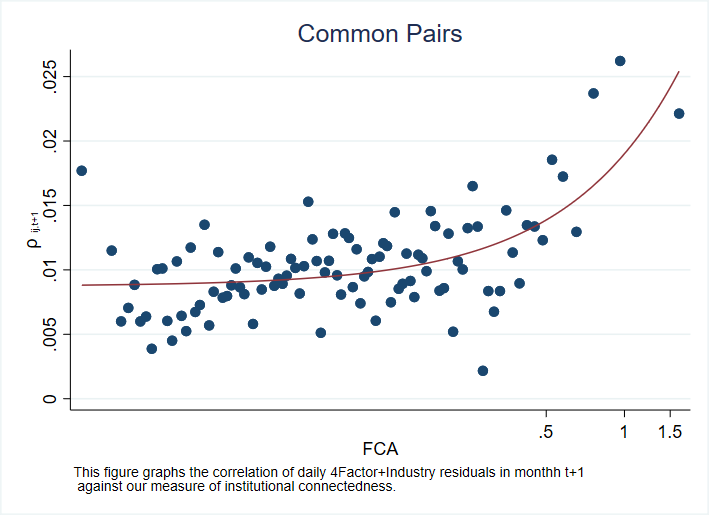
\includegraphics[width=0.7\linewidth]{"Output/mcorr50.eps"} 
		\caption{Future monthly correlation for different level of common ownership at this period }
		\label{mcorr50}
	\end{figure}
	\item 
	هم حرکتی دوره آینده را بر روی متغیر های مورد نظر برآورد می کنیم:
	\begin{equation}
\begin{split}
\rho_{ij,t+1} = & \text{ 	}\beta_0 + \beta_1* \text{FCA}^*_{ij,t} + \beta_2* \text{SameGroup}_{ij} \\
 &	+\beta_3* \text{FCA}^*_{ij,t} \times \text{SameGroup}_{ij}   \\
  & + \sum_{k=1} ^{n} \alpha_k*\text{Control}_{ij,t} + \varepsilon_{ij,t+1}
\end{split}
\label{model1}
\end{equation}
	
	\item
	برای هر ماه این معادله برآورد می شود و متوسط سری زمانی ضرایب به شیوه
	
	\lr{\cite{FamaMacBeth}}
	برآورد شده است
	\item
	این شیوه انتخاب شده است تا مشکلی با 
	\lr{cross-correlation}
	نداشته باشیم
	\item
	انحراف معیار هم به شیوه
	
	\lr{\cite{newey1987hypothesis}}
	اصلاح شده است تا 
	\lr{autocorrelation}
	را بر طرف کنید
	\item
	تا 4 دوره قبل را بر طرف می کنید
	($ 4(71/100)^{\frac{2}{9}} = 3.71 \sim 4 $)
	
	
\end{itemize}

\begin{itemize}
	\item 
	نتایج برآورد در جدول 
	\ref{mresult2part1}
	و
	\ref{mresult2part2}
	نشان داده شده است
	
\begin{itemize}
\item
جدول
\ref{mresult2part1}
\begin{itemize}

	\item 
	در دو ستون اول  اثر مالکیت مشترک بر روی هم حرکتی بررسی کرده ایم
	\item 
		در ستون 3 و 4 فقط گروه های کسب و کار را براورد کرده ایم حدودا $1.5$ درصد هم حرکتی افزایش پیدا می کند
	\item 
	اثر گروه کسب و کار بیشتر از مالکیت مشترک است
	\item 
	با اضافه کردن گروه کسب و کار و مالکیت مشترک، مالکیت مشترک اثر خود را از دست می دهد
\end{itemize}
	
\item
جدول
\ref{mresult2part2}
\begin{itemize}
	\item 
	مالکیت مشترک فقط در گروه های کسب و کار اثر دارد
	\item
	در دو ستون اخر هم بدون محدود کردن جامعه بودن در گروه را بررسی کرده ایم و یافتیم که در گروه کسب و کار مالکیت مشترک اهمیت دارد
	\item
	ستون آخر اثر ثابت گروه های کسب و کار را اضافه کردیم نتایج برقرار است
\end{itemize}
	
\end{itemize} 
\end{itemize}

	{\begin{table}[p]
	\centering
	\caption{Connected Co-movement}
	\label{mresult2part1}
	\resizebox{1\textwidth}{!}{
		\begin{LTR}
			\lr{{
\def\sym#1{\ifmmode^{#1}\else\(^{#1}\)\fi}
\begin{tabular}{l*{6}{c}}
\hline\hline
                    &\multicolumn{6}{c}{Dependent Variable:  Future Pairs's Comovement}                                                                 \\\cmidrule(lr){2-7}
                    &\multicolumn{1}{c}{(1)}         &\multicolumn{1}{c}{(2)}         &\multicolumn{1}{c}{(3)}         &\multicolumn{1}{c}{(4)}         &\multicolumn{1}{c}{(5)}         &\multicolumn{1}{c}{(6)}         \\
\hline
$ \text{MFCAP*} $   &     0.00600\sym{***}&     0.00328\sym{***}&                     &                     &     0.00104         &    0.000929         \\
                    &      (8.10)         &      (4.87)         &                     &                     &      (1.68)         &      (1.53)         \\
[1em]
SameGroup           &                     &                     &      0.0358\sym{***}&      0.0254\sym{***}&      0.0242\sym{***}&      0.0219\sym{***}\\
                    &                     &                     &      (9.99)         &      (8.45)         &      (8.21)         &      (7.02)         \\
[1em]
SameIndustry        &                     &      0.0267\sym{***}&                     &      0.0216\sym{***}&      0.0212\sym{***}&      0.0215\sym{***}\\
                    &                     &      (7.39)         &                     &      (6.81)         &      (6.72)         &      (6.80)         \\
[1em]
SameBM              &                     &      0.0224\sym{***}&                     &      0.0213\sym{***}&      0.0214\sym{***}&      0.0199\sym{***}\\
                    &                     &      (6.41)         &                     &      (6.09)         &      (6.16)         &      (5.77)         \\
[1em]
SameSize            &                     &      0.0123\sym{**} &                     &      0.0143\sym{***}&      0.0138\sym{***}&      0.0254\sym{***}\\
                    &                     &      (3.24)         &                     &      (3.85)         &      (3.71)         &      (5.56)         \\
[1em]
CrossOwnership      &                     &      0.0600\sym{***}&                     &      0.0300\sym{*}  &      0.0316\sym{*}  &      0.0377\sym{**} \\
                    &                     &      (5.50)         &                     &      (2.36)         &      (2.48)         &      (2.93)         \\
[1em]
Constant            &      0.0142\sym{***}&      0.0204\sym{***}&      0.0103\sym{***}&      0.0187\sym{***}&      0.0188\sym{***}&      0.0280\sym{***}\\
                    &     (12.80)         &      (8.91)         &      (9.42)         &      (7.99)         &      (8.04)         &      (9.43)         \\
\hline
PairType Control    &          No         &          No         &          No         &          No         &          No         &         Yes         \\
Observations        &      389591         &      389591         &      389591         &      389591         &      389591         &      389591         \\
\hline\hline  \end{tabular}}
}
		\end{LTR}
	}
\end{table}}

	{\begin{table}[p]
	\centering
	\caption{Connected Co-movement}
	\label{mresult2part2}
	\resizebox{1\textwidth}{!}{
		\begin{LTR}
			\lr{{
\def\sym#1{\ifmmode^{#1}\else\(^{#1}\)\fi}
\begin{tabular}{l*{4}{c}}
\hline\hline
                &\multicolumn{4}{c}{Dependent Variable: Future Pairs's co-movement'}        \\\cmidrule(lr){2-5}
                &\multicolumn{1}{c}{(1)}         &\multicolumn{1}{c}{(2)}         &\multicolumn{1}{c}{(3)}         &\multicolumn{1}{c}{(4)}         \\
\hline
$ \text{MFCAP*} $&  0.00944\sym{***}& 0.000397         & 0.000377         &-0.0000113         \\
                &   (7.24)         &   (0.68)         &   (0.65)         &  (-0.02)         \\
[1em]
Same Group      &                  &                  &  0.00624\sym{**} &  0.00549\sym{*}  \\
                &                  &                  &   (2.81)         &   (2.27)         \\
[1em]
 $ (\text{MFCAP}^*) \times {\text{SameGroup} }  $ &                  &                  &  0.00992\sym{***}&   0.0107\sym{***}\\
                &                  &                  &   (6.49)         &   (6.97)         \\
\hline
Observations    &    58337         &  1607659         &  1665996         &  1665996         \\
Sub-sample      &SameGroup         &   Others         &      All         &      All         \\
Group Effect    &       No         &       No         &       No         &      Yes         \\
Controls        &      Yes         &      Yes         &      Yes         &      Yes         \\
$ R^2 $         &   0.0112         & 0.000577         & 0.000898         &  0.00575         \\
\hline\hline
\multicolumn{5}{l}{\footnotesize \textit{t} statistics in parentheses}\\
\multicolumn{5}{l}{\footnotesize \sym{*} \(p<0.05\), \sym{**} \(p<0.01\), \sym{***} \(p<0.001\)}\\
\end{tabular}
}
}
		\end{LTR}
	}
\end{table}}


% \begin{landscape}
%
%	{\begin{table}[p]
%	\centering
%	\caption{Connected Co-movement}
%	\label{mresult2}
%	\resizebox{1.2\textwidth}{!}{
%		\begin{LTR}
%			\lr{{
\def\sym#1{\ifmmode^{#1}\else\(^{#1}\)\fi}
\begin{tabular}{l*{7}{c}}
\hline\hline
                &\multicolumn{7}{c}{Dependent Variable: Future Monthly Correlation of 4F+Industry Residuals}                                         \\\cmidrule(lr){2-8}
                &\multicolumn{1}{c}{(1)}         &\multicolumn{1}{c}{(2)}         &\multicolumn{1}{c}{(3)}         &\multicolumn{1}{c}{(4)}         &\multicolumn{1}{c}{(5)}         &\multicolumn{1}{c}{(6)}         &\multicolumn{1}{c}{(7)}         \\
\hline
Same Group      &   0.0138\sym{***}&   0.0128\sym{***}&                  &                  &  0.00978\sym{***}&  0.00458         &  0.00356         \\
                &   (5.76)         &   (6.29)         &                  &                  &   (4.29)         &   (1.43)         &   (1.11)         \\
[1em]
$ \text{FCA*} $ &                  &                  &  0.00405\sym{***}&  0.00375\sym{***}&  0.00296\sym{***}&  0.00258\sym{***}&  0.00273\sym{***}\\
                &                  &                  &   (4.94)         &   (5.12)         &   (3.77)         &   (3.53)         &   (3.51)         \\
[1em]
 $ (\text{FCA}^*) \times {\text{SameGroup} }  $ &                  &                  &                  &                  &                  &  0.00524\sym{**} &  0.00517\sym{**} \\
                &                  &                  &                  &                  &                  &   (3.21)         &   (3.18)         \\
\hline
Observations    &   388492         &   388492         &   388492         &   388492         &   388492         &   388492         &   388492         \\
Group Effect    &       No         &       No         &       No         &       No         &       No         &       No         &      Yes         \\
Controls        &       No         &      Yes         &       No         &      Yes         &      Yes         &      Yes         &      Yes         \\
$ R^2 $         & 0.000404         &  0.00200         & 0.000423         &  0.00201         &  0.00229         &  0.00245         &  0.00875         \\
\hline\hline
\multicolumn{8}{l}{\footnotesize \textit{t} statistics in parentheses}\\
\multicolumn{8}{l}{\footnotesize \sym{*} \(p<0.05\), \sym{**} \(p<0.01\), \sym{***} \(p<0.001\)}\\
\end{tabular}
}
}
%		\end{LTR}
%	}
%\end{table}}
% \end{landscape}
\FloatBarrier



\subsection{\lr{High level of common ownership}}
\begin{itemize}
	\item 
	با توجه به جدول 
	\ref{measureResults}
	گروه های کسب و کار به صورت مالکیت بالاتر نیز دارند 
	\item
	برای برطرف کردن این مسئله بررسی را محدود به مالکیت مشترک بالا کردیم
	\item
	با توجه به شکل 
	\ref{Qmcorr5subsample}
	بالاتر از کوارتر سوم داده به نظر می آید بیشترین تاثیر را در هم حرکتی دارد
	
	\begin{figure}[htbp]
		\centering  
		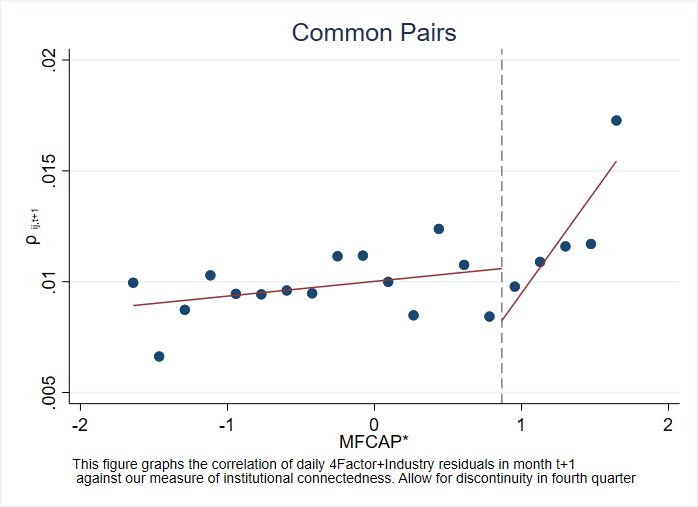
\includegraphics[width=0.6\linewidth]{"Output/Qmcorr5lrd.eps"}
		\caption{text}
		\label{Qmcorr5lrd}
	\end{figure}
	\begin{figure}[htbp]
		\centering  
		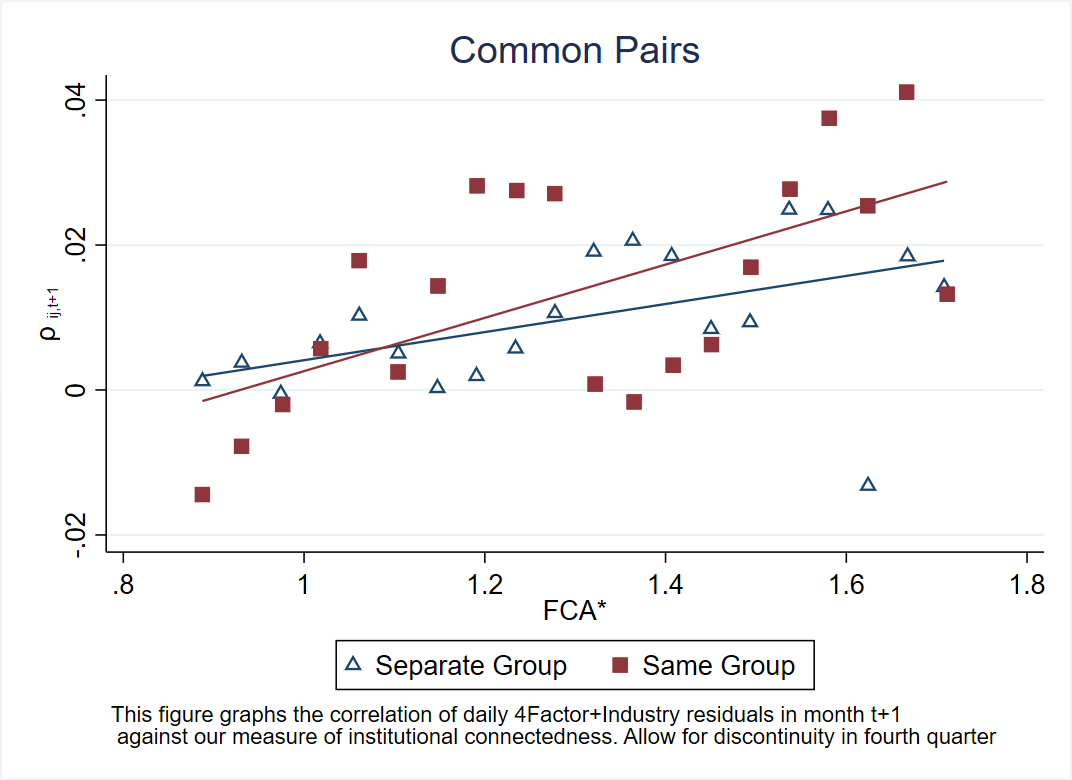
\includegraphics[width=0.45\linewidth]{"Output/Qmcorr5lrdbgsubsample.eps"}
		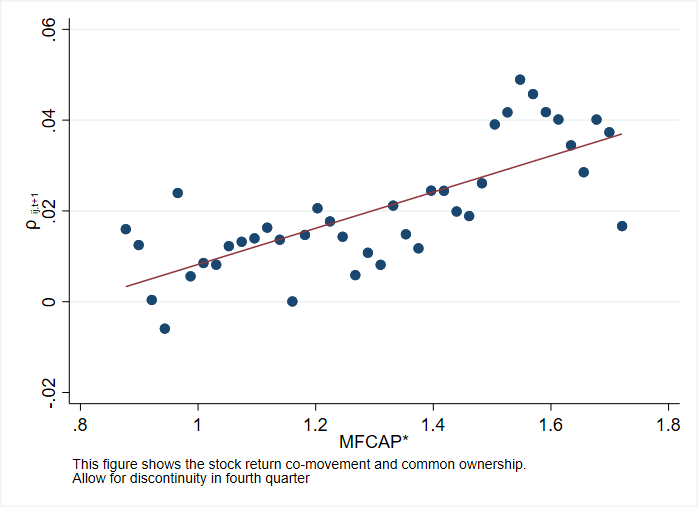
\includegraphics[width=0.45\linewidth]{"Output/Qmcorr5subsample.eps"}
		\caption{text}
		\label{Qmcorr5subsample}
	\end{figure}

	\item
	بررسی را محدود به جفت های دراای مالکیت زیاد کردیم و مدل 
	\ref{model1}
	را به شیوه گذشته برآورد کریدم
	\item
	نتایج در جدول 
	 \ref{QTimemresult2subsample}
	 نتایج را نشان داده است
\lr{\begin{LTR}
			 \begin{table}[htbp]
	 	\centering
	 	\caption{\scriptsize Estimation results for high level of common ownership}
	 	\label{QTimemresult2subsample}
	 	\resizebox{\textwidth}{!}{
	 		{
\def\sym#1{\ifmmode^{#1}\else\(^{#1}\)\fi}
\begin{tabular}{l*{7}{c}}
\hline\hline
                &\multicolumn{7}{c}{Dependent Variable:  Future Pairs's Comovement}                                                                  \\\cmidrule(lr){2-8}
                &\multicolumn{1}{c}{(1)}         &\multicolumn{1}{c}{(2)}         &\multicolumn{1}{c}{(3)}         &\multicolumn{1}{c}{(4)}         &\multicolumn{1}{c}{(5)}         &\multicolumn{1}{c}{(6)}         &\multicolumn{1}{c}{(7)}         \\
\hline
SameGroup       &   0.0254\sym{***}&                  &   0.0249\sym{***}&                  &                  &  0.00477         &  0.00252         \\
                &   (8.45)         &                  &   (8.21)         &                  &                  &   (1.32)         &   (0.66)         \\
[1em]
$ (\text{MFCAP} > \text{Larger than 75th Percentile}) $ &                  &  0.00660\sym{***}& 0.000777         &   0.0230\sym{***}& -0.00258\sym{*}  & -0.00157         &-0.000513         \\
                &                  &   (5.48)         &   (0.73)         &   (7.09)         &  (-2.00)         &  (-1.29)         &  (-0.46)         \\
[1em]
 $ (\text{MFCAP} > Q3[\text{MFCAP}]) \times {\text{SameGroup}} $ &                  &                  &                  &                  &                  &   0.0248\sym{***}&   0.0237\sym{***}\\
                &                  &                  &                  &                  &                  &   (7.24)         &   (7.34)         \\
\hline
Sub-sample      &      All         &      All         &      All         &SameGroup         &   Others         &      All         &      All         \\
Controls        &      Yes         &      Yes         &      Yes         &      Yes         &      Yes         &      Yes         &      Yes         \\
Business Group FE&       No         &       No         &       No         &       No         &       No         &       No         &      Yes         \\
Observations    &   389591         &   389591         &   389591         &    47076         &   342515         &   389591         &   389591         \\
\hline\hline
\multicolumn{8}{l}{\footnotesize \textit{t} statistics in parentheses}\\
\multicolumn{8}{l}{\footnotesize \sym{*} \(p<0.05\), \sym{**} \(p<0.01\), \sym{***} \(p<0.001\)}\\
\end{tabular}
}

	 	}
	 \end{table}
\end{LTR}}
	\begin{itemize}
		\item 
		همچنان نتایج گذشته تایید شده است
		\item 
	مالکیت مشترک صرفا در گروه های کسب و کار اهمیت دارد 
		\item 
		گروه های کسب و کار بیشترین تاثیر را در میان سطح زیاد مالیکت مشترک دارد
		\item 
		ممکن است جفت های دارای مالکیت بالا تفاوت بنیادی با دیگر جفت ها داشته باشند 
		\begin{itemize}
			\item 
			در شکل 
			\ref{QarterSummary}
			متوسط کنترل های تعریف شده نشان داده شده است
			\begin{figure}[htbp]
				\centering  
				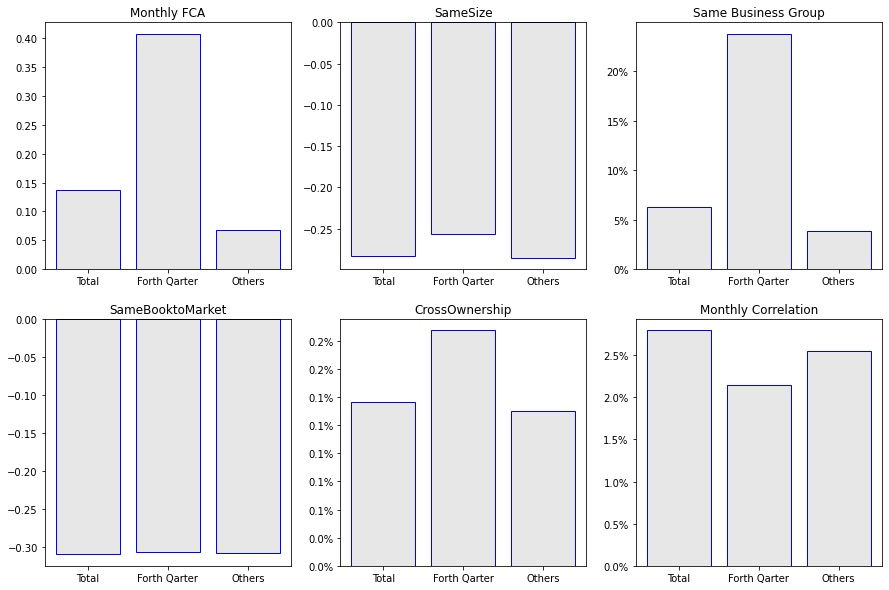
\includegraphics[width=0.85\linewidth]{"Output/QarterSummary.eps"}
				\caption{Pairs' characteristics for the pairs with high level of common ownership}
				\label{QarterSummary}
			\end{figure}
		\item
		تفاوت چشمگیری نسبت به بقیه جامعه ندارند
		\end{itemize}
	\end{itemize}
	
	
\end{itemize}


\FloatBarrier

\subsection{All Pairs}
\begin{itemize}
	\item 
	اگر گروه های کسب و کار اهمیت داشته باشند نیاز نیست تا محاسبات را محدود به شرکت های دارای مالک مشترک کنیم
	\item
	همه جفت های بازار را تشکیل می دهیم
	\item
	زمانی که مالکیت مشترک وجود ندارد مالکیت مشترک را برابر صفر قرار می دهیم و اگر مالکیت مشترک داشته باشند میزان ارن را محاسبه می کنیم
	\item
	برای همه جفت ها مدل 
	\ref{model1}
	را به شیوه گذشته برآورد می کنیم
	\item
	نتایج در جدول 
	\ref{AllPairs}
	نشان داده شده است
	\begin{itemize}
		\item 
		در ستون اول عضویت در گروه کسب و کار را نشان می دهد که علامت و مقدار برآورد قبلی را نشان می دهد
		\item 
		در ستون2 نیز برای سطح مالکیت مشترک بررسی شده است و نتایج قبلی تایید شده است
		\item 
		در میان گروه کسب و کار سطح مالکیت مشترک تاثیر چندانی ندارد
		\item
		درمیان جفت های بیرون گروه کسب و کار نیز سطح مالکیت مشترک اهمیت دارد که می تواند صرفا اهمیت مالکیت مشترک در پیش بینی هم حرکتی قیمت شرکت ها را نشان دهد.
			\begin{table}[htbp]
					%	\centering
					\caption{Non-connected Co-movement}
					\label{AllPairs}
					\resizebox{1\textwidth}{!}{
					\begin{LTR}
						\lr{	{
\def\sym#1{\ifmmode^{#1}\else\(^{#1}\)\fi}
\begin{tabular}{l*{7}{c}}
\hline\hline
                &\multicolumn{7}{c}{Dependent Variable: Future Pairs' co-movement}                                                                   \\\cmidrule(lr){2-8}
                &\multicolumn{1}{c}{(1)}         &\multicolumn{1}{c}{(2)}         &\multicolumn{1}{c}{(3)}         &\multicolumn{1}{c}{(4)}         &\multicolumn{1}{c}{(5)}         &\multicolumn{1}{c}{(6)}         &\multicolumn{1}{c}{(7)}         \\
\hline
SameGroup       &   0.0156\sym{***}&                  &   0.0158\sym{***}&                  &                  &   0.0138\sym{***}&   0.0131\sym{***}\\
                &   (9.84)         &                  &  (10.22)         &                  &                  &   (8.27)         &   (7.68)         \\
[1em]
$ \text{MFCAP*}  $&                  &-0.0000723         &-0.000277         &  0.00169         &-0.000322\sym{*}  &-0.000390\sym{**} &-0.000427\sym{*}  \\
                &                  &  (-0.44)         &  (-1.80)         &   (1.42)         &  (-2.19)         &  (-2.70)         &  (-2.29)         \\
[1em]
 $ (\text{MFCAP}^*) \times {\text{SameGroup} }  $ &                  &                  &                  &                  &                  &  0.00313\sym{**} &  0.00364\sym{**} \\
                &                  &                  &                  &                  &                  &   (2.80)         &   (3.34)         \\
\hline
Controls        &      Yes         &      Yes         &      Yes         &      Yes         &      Yes         &      Yes         &      Yes         \\
Sub-Sample      &    Total         &    Total         &    Total         &SameGroups         &   Others         &    Total         &    Total         \\
Business Group FE&       No         &       No         &       No         &       No         &       No         &       No         &      Yes         \\
Observations    &  6018646         &  6018646         &  6018646         &   114526         &  5904120         &  6018646         &  6018646         \\
\hline\hline
\multicolumn{8}{l}{\footnotesize \textit{t} statistics in parentheses}\\
\multicolumn{8}{l}{\footnotesize \sym{*} \(p<0.05\), \sym{**} \(p<0.01\), \sym{***} \(p<0.001\)}\\
\end{tabular}
}

					}
					\end{LTR}}
				\end{table}
	\end{itemize}
	
\end{itemize}






\FloatBarrier




%\subsection{\lr{Size effect}}
%\begin{itemize}
%	\item 
%	مقاله
%	\lr{\cite{AntonPolk}}
%	بررسی اصلی را محدود به شرکت های بزرگ کرده بود
%	\item 
%	بررسی می کنیم آیا اثر به اندازه شرکت ها وابسته است یا خیر
%	\item 
%	شرکت های بزرگتر از میانه ارزش بازار را شرکت های بزرگ دسته بندی می کنیم
%	\item 
%	سه نوع جفت تولید می شود جفت های بزرگ، ترکیبی و کوچک
%	\item 
%	که آنالیز 
%	\lr{\cite{AntonPolk}}
%	فقط برای جفت های بزرگ صورت گرفته است
%	\item 
%	شکل 
%	\ref{mcorrPairType}
%	نشان داده شده است
%	\begin{figure}[htbp]
%		\centering  
%		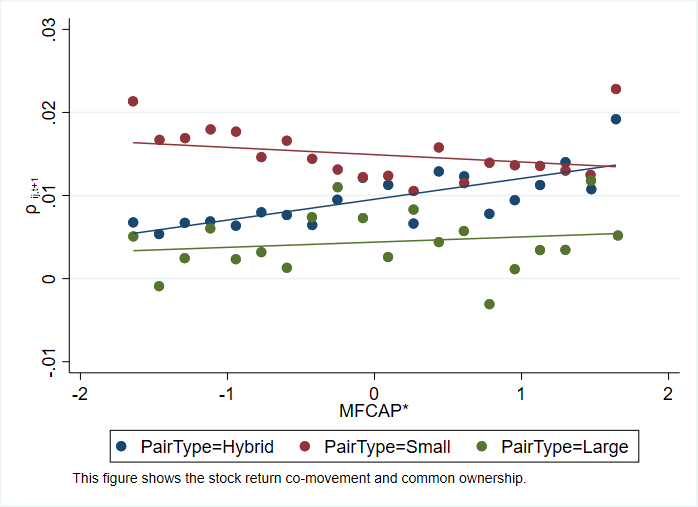
\includegraphics[width=0.7\linewidth]{"Output/mcorrPairType.eps"}
%		\caption{text}
%		\label{mcorrPairType}
%	\end{figure}
%	\item 
%	در ابتدا انالیز اصلی را برای جفت های دارای مالک مشترک انجام دادیم
%	\item
%	جدول  
%	\ref{Qmresult4}
%	نشان داده است
%		\begin{LTR}
%		\lr{\begin{table}[htbp]
%				\centering
%				\caption{text}
%				\label{Qmresult4}
%				\resizebox{1\textwidth}{!}{
%					{
\def\sym#1{\ifmmode^{#1}\else\(^{#1}\)\fi}
\begin{tabular}{l*{8}{c}}
\hline\hline
                &\multicolumn{8}{c}{Dependent Variable: Future Monthly Correlation of 4F+Ind. Res.}                                                                     \\\cmidrule(lr){2-9}
                &\multicolumn{1}{c}{(1)}         &\multicolumn{1}{c}{(2)}         &\multicolumn{1}{c}{(3)}         &\multicolumn{1}{c}{(4)}         &\multicolumn{1}{c}{(5)}         &\multicolumn{1}{c}{(6)}         &\multicolumn{1}{c}{(7)}         &\multicolumn{1}{c}{(8)}         \\
\hline
$ \text{FCA*} $ & 0.000377         & 0.000698         &-0.000175         &  0.00199\sym{***}&  0.00177\sym{**} & -0.00151         & -0.00177         &-0.0000771         \\
                &   (0.65)         &   (1.25)         &  (-0.31)         &   (3.56)         &   (3.00)         &  (-1.58)         &  (-1.84)         &  (-0.14)         \\
[1em]
Same Group      &  0.00624\sym{**} &   0.0102\sym{***}& -0.00153         &   0.0117\sym{***}&  0.00661\sym{*}  &   0.0366\sym{***}&   0.0268\sym{***}&  0.00750\sym{***}\\
                &   (2.81)         &   (3.95)         &  (-0.53)         &   (3.76)         &   (2.15)         &  (10.31)         &   (6.57)         &   (3.53)         \\
[1em]
 $ (\text{FCA}^*) \times {\text{SameGroup} }  $ &  0.00992\sym{***}&                  &   0.0134\sym{***}&                  &  0.00599\sym{*}  &                  &   0.0123\sym{***}&   0.0105\sym{***}\\
                &   (6.49)         &                  &   (4.80)         &                  &   (2.34)         &                  &   (4.17)         &   (6.72)         \\
\hline
Observations    &  1665996         &   346170         &   346170         &   693728         &   693728         &   626098         &   626098         &  1665996         \\
Controls        &      Yes         &      Yes         &      Yes         &      Yes         &      Yes         &      Yes         &      Yes         &      Yes         \\
Sub-sample      &All Firms         &Big Firms         &Big Firms         &Big \& Small Firms         &Big \& Small Firms         &Small Firms         &Small Firms         &All Firms         \\
Pair Size FE    &       No         &       No         &       No         &       No         &       No         &       No         &       No         &      Yes         \\
$ R^2 $         & 0.000898         &  0.00193         &  0.00232         &  0.00135         &  0.00149         &  0.00180         &  0.00198         &  0.00130         \\
\hline\hline
\multicolumn{9}{l}{\footnotesize \textit{t} statistics in parentheses}\\
\multicolumn{9}{l}{\footnotesize \sym{*} \(p<0.05\), \sym{**} \(p<0.01\), \sym{***} \(p<0.001\)}\\
\end{tabular}
}

%				}
%		\end{table}}
%	\end{LTR}
%	\begin{itemize}
%		\item 
%		در جفت های بزرگ و کوچک نتایج با نتایج اولیه همسان است
%		\item 
%		در حفت های ترکیبی همچنان مالکیت مشترک و عضویت در گروه کسب و کار اهمیت دارد
%		
%	\end{itemize}
%	\item
%	سپس انالیز را برای تمام  جفت های بازار  انجام دادیم
%	\item
%	جدول  
%	\ref{Qmresult4AllPairs}
%	نشان داده است
%	\begin{LTR}
%		\lr{	\begin{table}[htbp]
%				\centering
%				\caption{text}
%				\label{Qmresult4AllPairs}
%				\resizebox{1\textwidth}{!}{
%					{
\def\sym#1{\ifmmode^{#1}\else\(^{#1}\)\fi}
\begin{tabular}{l*{8}{c}}
\hline\hline
                &\multicolumn{8}{c}{Dependent Variable: Future Monthly Correlation of 4F+Ind. Res.}                                                                     \\\cmidrule(lr){2-9}
                &\multicolumn{1}{c}{(1)}         &\multicolumn{1}{c}{(2)}         &\multicolumn{1}{c}{(3)}         &\multicolumn{1}{c}{(4)}         &\multicolumn{1}{c}{(5)}         &\multicolumn{1}{c}{(6)}         &\multicolumn{1}{c}{(7)}         &\multicolumn{1}{c}{(8)}         \\
\hline
SameGroup       &   0.0134\sym{***}&  0.00954\sym{***}&  0.00853\sym{***}&   0.0136\sym{***}&   0.0118\sym{***}&   0.0314\sym{***}&   0.0267\sym{***}&   0.0138\sym{***}\\
                &   (7.81)         &   (4.63)         &   (3.71)         &   (7.35)         &   (6.46)         &  (10.19)         &   (7.93)         &   (8.27)         \\
[1em]
$ \text{FCA*} $ & 0.000408\sym{*}  &-0.0000120         &-0.000115         & 0.000514\sym{*}  & 0.000401         & -0.00143\sym{***}& -0.00154\sym{***}&-0.000390\sym{**} \\
                &   (2.11)         &  (-0.05)         &  (-0.47)         &   (2.09)         &   (1.67)         &  (-3.86)         &  (-3.97)         &  (-2.70)         \\
[1em]
 $ (\text{FCA}^*) \times {\text{SameGroup} }  $ &  0.00247\sym{*}  &                  &  0.00178         &                  &  0.00272         &                  &  0.00545\sym{**} &  0.00313\sym{**} \\
                &   (2.15)         &                  &   (1.30)         &                  &   (1.59)         &                  &   (3.38)         &   (2.80)         \\
\hline
Observations    &  6018646         &  1753614         &  1753614         &  2992221         &  2992221         &  1272811         &  1272811         &  6018646         \\
Controls        &      Yes         &      Yes         &      Yes         &      Yes         &      Yes         &      Yes         &      Yes         &      Yes         \\
Sub-sample      &All Firms         &Large Firms         &Large Firms         &Hybrid Firms         &Hybrid Firms         &Small Firms         &Small Firms         &All Firms         \\
Pair Size FE    &       No         &       No         &       No         &       No         &       No         &       No         &       No         &      Yes         \\
$ R^2 $         & 0.000515         & 0.000796         & 0.000860         & 0.000688         & 0.000735         &  0.00191         &  0.00199         & 0.000829         \\
\hline\hline
\multicolumn{9}{l}{\footnotesize \textit{t} statistics in parentheses}\\
\multicolumn{9}{l}{\footnotesize \sym{*} \(p<0.05\), \sym{**} \(p<0.01\), \sym{***} \(p<0.001\)}\\
\end{tabular}
}

%				}
%		\end{table}}
%	\end{LTR}
%	\begin{itemize}
%	\item 
%	برای جفت های بزرگ صرفا گروه های کسب و کار اهمیت دارد 
%	\item 
%	برای جفت های بزرگ اصلا مالکیت مشترک اهمیت ندارد
%	\item 
%	در جفت های کوجک گروه کسب و کار اثر مثبت و مالکیت مشترک بیرون گروه کسب و کار اثر منفی دارد 
%	\item
%	در جفت های ترکیبی نیز مالکیت مشترک اثر کمتری از گروه کسب و کار دارد
%	
%\end{itemize}
%\end{itemize}
%		
%
%
%	
	





\FloatBarrier

